
% \usepackage{geometry}
\usepackage[dvipdfmx]{graphicx}
\usepackage{ascmac}
\usepackage{amsmath}
\usepackage{amssymb}
\usepackage{minted}
\usepackage{listings}
% \usepackage[utf8]{inputenc}
% \usepackage{listingsutf8}
\usepackage{newfloat} % newfloat パッケージを読み込む
\usepackage{caption}
\usepackage{float}
\usepackage{fix-cm}
\usepackage{svg}
\usepackage{enumitem}

\usepackage{hyperref}
% for hyperref
\usepackage{pxjahyper}
\hypersetup{
    dvipdfmx,
	colorlinks=false, % リンクに色をつけない設定
	bookmarks=true, % 以下ブックマークに関する設定
	bookmarksnumbered=true,
	pdfborder={0 0 0},
	bookmarkstype=toc
}

% \lstset{
%   basicstyle={\ttfamily},
%   identifierstyle={\small},
%   inputencoding=auto,
%   commentstyle={\small\sffamily},
%   keywordstyle={\small\bfseries},
%   ndkeywordstyle={\small},
%   stringstyle={\small\ttfamily},
%   frame={tb},
%   breaklines=true,
%   columns=[l]{fullflexible},
%   numbers=left,
%   % xrightmargin=0zw,
%   % xleftmargin=3zw,
%   numberstyle={\scriptsize},
%   firstnumber=auto,
%   stepnumber=1,
%   numbersep=5pt,
%   lineskip=1ex
% }

% 新しい浮動体「listing」を定義
\DeclareFloatingEnvironment[
    fileext=lol,       % List of Listings ファイルの拡張子 (List of Listings を作成する場合)
    name=Listing,      % キャプションの接頭辞 (例: "Listing 1")
    placement={!htbp}, % フロートの配置オプション (お好みで調整してください)
    within=section     % 番号付けをセクションごとにする場合 (例: Listing 1.1) (任意、不要なら削除)
]{program}

\setminted{
  mathescape,              % 数式モードへのエスケープを許可 (必要なら)
  % basicstyle やフォント関連
  fontsize=\small,         % 全体のフォントサイズ (listings の \small に合わせる試み)
                           % \ttfamily は minted のデフォルトに近いが、日本語対応の等幅フォントを
                           % LaTeX 側で \ normaalfont や \ttdefault に設定しておくのが理想
  % frame
  frame=lines,             % 上下に線を引く frame=tb に近いものとして lines (上下左右に線)
  framesep=2mm,            % 枠線とコードの間隔 (調整が必要)
  % breaklines
  breaklines=true,         % 自動折り返し
  % numbers
  linenos=true,            % 行番号を左に表示
  firstnumber=auto,        % 行番号を開始行に合わせる
  numbersep=5pt,           % 行番号とコードの間隔
  % stepnumber=1,          % linenos=true で通常1ステップ
  % highlight と Pygments スタイル
  % minted では Pygments のスタイルを使います。
  % style=friendly のようにスタイル名を指定できます。
  % デフォルトのスタイルでキーワードが太字になるか確認。
  % commentstyle や keywordstyle の LaTeX コマンド直接指定はできません。
  % Pygments のスタイルでこれらがどのように見えるか確認し、
  % 必要ならカスタムスタイルを作るか、別の既存スタイルを選びます。
}

\title{計算量について}
\author{佐藤謙成}
\institute{KUT-PG}

\begin{document}
\begin{frame}
    \titlepage
\end{frame}

\begin{frame}{目次}
    \tableofcontents[]
\end{frame}


\section{計算量(オーダー)}
\begin{frame}{オーダー記法}
    \begin{block}{オーダー記法とは}
        アルゴリズムの計算量を評価するための記法. $t$ を時間とすると,$O(t)$で表すことができる. $t$は小さい方が計算量が少ないため,評価は高くなる.
        \begin{itemize}
            \item アルゴリズムによって所要時間が異なる
            \item 良いアルゴリズムの場合は解決したい問題の規模が大きくなっても対抗可能である.
        \end{itemize}
        
        以下は, $t$に入る代表格である.
        \begin{align*}
            \log{n} < \sqrt{n} < n < n\log{n} < n^2 < n^3 < \cdots < 2^n < n!
        \end{align*}
        できるだけ $\log{n} $になるようにアルゴリズムを組んでいきたい.
    \end{block}
    
    \begin{block}{オーダー記法($t$)の決め方}
        \begin{enumerate}
            \item アルゴリズムの時間計算量を入力サイズ $n$ を用いた関数で表す.
            \item その関数の中で主要項\footnote{$n$ が一番大きいもの}を見つける.
            \item 主要項の係数を削除した関数が $f(n)$である時,アルゴリズムの時間計算量は $O(f(n))$であるという.
        \end{enumerate}
    \end{block}
\end{frame}

\begin{frame}{実行時間}
    アルゴリズムの実行時間に関して,以下の語句で表現される.
    \begin{enumerate}
        \item 時間計算量
        \item 最良時間計算量
        \item 最悪時間計算量
        \item 領域計算量
        \item 平均時間計算量
    \end{enumerate}
    \begin{block}{最良時間計算量}
        最も速くそのアルゴリズムを実行できる入力の時間計算量.
    \end{block}
    \begin{block}{最悪時間計算量}
        最も時間のかかる入力に対する時間計算量. .
    \end{block}
    \begin{block}{平均時間計算量}
        入力データがランダムに分布している場合の計算時間を示す.
    \end{block}
    \begin{block}{領域計算量}
        アルゴリズムを実行する際にどれだけのメモリ(領域)が必要かを表す.
    \end{block}
\end{frame}

\begin{frame}{計算量の評価}
\begin{block}{}
計算量の評価は以下の通りとなる.
    \begin{align*}
    \log{n} < \sqrt{n} < n < n\log{n} < n^2 < n^3 < \cdots < 2^n < n!
    \end{align*}
\end{block}
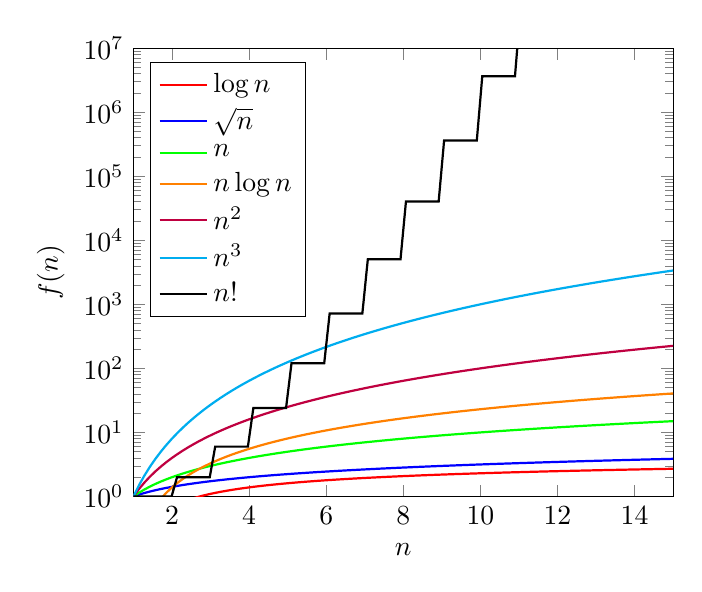
\begin{tikzpicture}
    \begin{axis}[
        xlabel={$n$},
        ylabel={$f(n)$},
        legend pos=north west,
        ymode=log,                % y軸に対数スケールを使用
        xmin=1, xmax=15,          % X軸の範囲(表示用)
        ymin=1, ymax=1e7,         % Y軸の範囲(表示用)、n! のために ymax を増加
        samples=100,              % プロット用のサンプル数
        domain=1:15,              % xの計算ドメイン(nの値は1から10)
        legend cell align={left}, % 凡例の項目を左揃えにする
        % grid=both,              % グリッドが必要な場合はコメントを外す
    ]
    \addplot[thick, color=red]   {ln(x)};        \addlegendentry{$\log{n}$}
    \addplot[thick, color=blue]  {sqrt(x)};      \addlegendentry{$\sqrt{n}$}
    \addplot[thick, color=green] {x};            \addlegendentry{$n$}
    \addplot[thick, color=orange]{x*ln(x)};      \addlegendentry{$n\log{n}$}
    \addplot[thick, color=purple]{x^2};          \addlegendentry{$n^2$}
    \addplot[thick, color=cyan]  {x^3};          \addlegendentry{$n^3$}
    \addplot[thick, color=black]  {x!};       \addlegendentry{$n!$}
    \end{axis}
\end{tikzpicture}
\end{frame}

\begin{frame}{基本演算での時間計算量}
\begin{block}{}
        \begin{itemize}
        \item 算術演算
        \item 論理演算
        \item 入出力の命令
    \end{itemize}
    これらの基本演算の時間計算量は $O(1)$(定数時間)となる.
\end{block}
\end{frame}

\begin{frame}{時間計算量の例.1}
    以下のアルゴリズムの時間計算量を求めていく.
    \begin{exampleblock}{アルゴリズムA}
        $10n^2 + 100n + 10000$
    \end{exampleblock}
    \begin{exampleblock}{アルゴリズムB}
        $n^4 - n^3 + 100$
    \end{exampleblock}

        \begin{block}{再掲}
        \begin{enumerate}
            \item アルゴリズムの時間計算量を入力サイズ $n$ を用いた関数で表す.
            \item その関数の中で主要項\footnote{$n$ が一番大きいもの}を見つける.
            \item 主要項の係数を削除した関数が $f(n)$である時,アルゴリズムの時間計算量は $O(f(n))$であるという.
        \end{enumerate}
    \end{block}
\end{frame}

\begin{frame}[fragile]{時間計算量の例.2}
以下のコードを元に時間計算量を求めていきたい.(計算量オーダーは,最悪時間計算量について考えるのが基本である.)
    \lstinputlisting{./code/order/for.txt}
\begin{exampleblock}{}
    \begin{itemize}
        \item if文の時間計算量は, $O(1)$である.
        \item 外側のfor文の繰り返し回数は, $n - 1$回.
        \item 内側のfor文の繰り返し回数は, $n - i$回.
    \end{itemize}
    このアルゴリズムの時間計算量は,
    \begin{align*}
        O(1) \times \dfrac{n(n - 1)}{2} = O(n^2)
    \end{align*}
\end{exampleblock}
\end{frame}

\begin{frame}{計算量の使い方}
    実際の問題をに対してアルゴリズムを設計する時の考え方について考えていく.
    
    通常の計算機では 1 秒間に処理できるfor文のループの回数は, $ 10^8 $ 回程度である.
    (Atcoderでは通常,制限時間が2秒間であるので命令実行の回数は $2 \times 10^8$ 回程度である.)
    \[
        \begin{array}{ *{7}{l}}
        \log{n} & n & n\log{n} & n^2 & n^3 & 2^n & n! \\
        \hline
        2 & 5 & 12 & 25 & 130 & 30 & 120 \\
        3 & 10 & 33 & 100 & 1000 & 1024 & 362880 \\
        4 & 15 & 59 & 225 & 3375 & 32768 & - \\
        4 & 20 & 86 & 400 & 8000 & 1048576 & - \\
        5 & 25 & 116 & 625 & 15625 & - & - \\
        5 & 30 & 147 & 900 & 27000 & - & - \\
        7 & 100 & 664 & 10000 & 1000000 & - & -
        \end{array}
    \]
\end{frame}
\end{document}
